\documentclass[a4paper,11pt,openany]{book} % bez prazdnych stran
%\documentclass[a4paper,11pt]{book} % s prazdnymi stranami, aby kapitola zacinala na neparnej, vhodne pre tlac

% definovanie kompilatora (magic comment):
% !TeX program = xelatex

% ============== PREAMBULA ==============
% (nacitanie balikov a podobne)
% ============== PREAMBULA ==============
% (nacitanie balikov a podobne)
% Ctrl+klik na balik zobrazi dokumentaciu k baliku (v TeXstudiu)
% Je tu vela uzitocnych balikov ak ale nejaky nepotrebujete, zakomentujte ho

%definovanie verzie dokumentu (pdf/tlacena)
\usepackage{etoolbox}
\newbool{printVersion} % premenna pre volbu verzie
%\booltrue{printVersion} % tlacena: odkomentovat, pdf: nechat zakomentovanie


% geometria a formatovanie stran
\pagestyle{plain} % defaultny styl stran (plain/headings/empty/myheadings)
\ifbool{printVersion}{
	\usepackage[top=2.5cm, bottom=2.5cm, left=3.5cm, right=2cm]{geometry} % odporucane okraje
}{
	\usepackage[top=2.5cm, bottom=2.5cm, left=2.75cm, right=2.75cm]{geometry} % okraje vhodnejsie do pdf (rovnaka sirka vlavo/vpravo) 
}

% jazyk
\usepackage[main=slovak,english]{babel}  % primarny jazyk: SK, dalsie jazyky: EN


% bibliografia
\usepackage[style=iso-numeric,backend=bibtex,giveninits=true,sorting=nyt]{biblatex}
\addbibresource{literatura.bib}


% fromatovanie
\usepackage{indentfirst} % odsadenie prveho odstavca
\usepackage{enumitem} % číslovanie ((a),(b),(c),... i), ii), iii),...)
\usepackage[small]{caption} % male popisy obrazkov


% grafika
\usepackage{graphicx} % obrazky
\usepackage{subcaption} % podobrazky (subfigure)
\graphicspath{ {./figures/} } % priecinok s obrazkami
\usepackage{wrapfig} % obrazky obtekane textom
\usepackage[dvipsnames]{xcolor} % farby (dvipsnames pridava dalsie farby)
\usepackage{colortbl} % farebne tabulky
\usepackage{multirow} % treba pre merge-ovanie budniek v tabulkach

\usepackage{pdfpages} % vlozenie stran z ineho pdf (musi byt za graphics)


% matematika
\usepackage{mathtools} % rozsirenie zakladneho matematickeho balika amsmath
\usepackage{amssymb} % dalsie symboly a fonty (napriklad pre mnozinu realnych cisel)
\usepackage[locale=DE]{siunitx} % jednotky SI

% Definície, Vety, Dôkazy...
\usepackage{amsthm}
\theoremstyle{definition}
\newtheorem{thm}{Veta}[chapter]
\newtheorem{defn}[thm]{Definícia}
\newtheorem{lem}[thm]{Lemma}
\newtheorem{cor}[thm]{Dôsledok}
\newtheorem{rem}[thm]{Poznámka}
\newtheorem{exmp}[thm]{Príklad}


% pseudokod a kod
\usepackage[czech]{algorithm2e} % pseudokody/algoritmy
\usepackage{listings} % vkladanie kodu


% hyperreferencia
\ifbool{printVersion}{
	% hyperreferencia v tlacenej verzii
	\usepackage[hidelinks]{hyperref} % hyperreferencia
}{
	% hyperreferencia v pdf verzii
	\usepackage{hyperref} % hyperreferencia
	\hypersetup{colorlinks, % farby linkov
		citecolor = red,
		linkcolor = blue,
		urlcolor = blue}
}

\usepackage{placeins}
\usepackage{float}
\usepackage{subcaption}

% Ked uz je praca dlha, pre urychlenie kompilacie sa oplati vkladat len niektore kapitoly
%\includeonly{
	%%	Uvod,
	%%	Kapitola1,
	%%	Kapitola2,
	%	Kapitola3,
	%%	Zaver
	%}


% ============== DOKUMENT ==============
\begin{document}
	% ====== Uvodne casti ======
	\pagestyle{empty}
	% Do tlacenej verzie v kniznej vazbe sa obalka neviaze, sluzi ako predloha pevnej obalky. Do tepelnej vazby sa viaze.

\begin{center}
	\textsc{\LARGE
		Slovenská technická univerzita v Bratislave\\
		\vspace{10pt}
		Stavebná fakulta}\\
	
	\begin{flushleft}
		Evidenčné číslo: SvF-
	\end{flushleft}
	\vfill
	
	\textsc{\LARGE
		Názov práce}\\ 
	\vspace{10pt}
	{\Large
		Bakalárska práca}
\end{center}

\vfill

{\Large
	\noindent \textbf{2022}
	\hfill \textbf{Meno Priezvisko} % pripadne tituly
}

\ifbool{printVersion}{ % prazdna strana
	\newpage
	\
	\newpage
}
\

	\setcounter{page}{1}
	\newgeometry{top=2.5cm, bottom=2.5cm, left=2.25cm, right=2.25cm}
\thispagestyle{empty}

\begin{center}% logo SvF STU
	
\includegraphics[height=2.8cm]{figures/STU-SvF-nfh}
\end{center}
\vspace{1cm}

\begin{flushright}
	\text{\Large
		Študentská vedecká konferencia}\\
	\text{\Large
		Akademický rok 2024/2025}
\end{flushright}
\vspace{3cm}

\begin{center}
	\textsc{\LARGE Modelovanie rozdelenia pravdepodobnosti zmesi}\\
	\vspace{2pt}
	\textsc{\LARGE spojitých a diskrétnych náhodných premenných}
\end{center}
\vfill

\noindent
\begin{tabular}{ll}
	Meno a priezvisko študenta, ročník, odbor: & Adam Harmaniak, 3. ročník, B-MPM\\
	Vedúci práce: & doc. Ing. Tomáš Bacigál, PhD.\\
	Katedra / Ústav: & Katedra matematiky a deskriptívnej geometrie
\end{tabular}
\vspace{3cm}

\begin{center}
	\Large Bratislava 9. apríla 2025 % upravit na datum konania SVK
\end{center}
\restoregeometry
\newpage

\ifbool{printVersion}{ % prazdna strana
	\thispagestyle{empty}
	\
	\newpage
}
\


	\includepdf[pages=-,pagecommand={}]{documents/zadanie_AIS.pdf} % stiahnete z AIS
	% Pre vlozenie pokynov na vypracovanie, odkomentujte nasledujuce 3 riadky
%	\ifbool{printVersion}{\cleardoublepage}
%	
%	\includepdf[pages=-,pagecommand={}]{documents/Pokyny_BP_2015.pdf}
	\ifbool{printVersion}{
	\cleardoublepage % ak to vychadza na parnu stranu, vlozi sa prazdna strana
}

\
\vfill

\subsection*{Čestné prehlásenie}

Prehlasujem, že som túto záverečnú prácu vypracoval/a samostatne pod vedením vedúceho záverečnej práce, s~použitím literatúry uvedenej v~zozname použitej literatúry.

\vspace{10pt}

\noindent Bratislava 6. 5. 2022 \hfil
\newline

\begin{flushright}
	Meno Priezvisko $\qquad$
\end{flushright}

	\ifbool{printVersion}{
	\cleardoublepage % ak to vychadza na parnu stranu, vlozi sa prazdna strana
}

\
\vfill

\subsection*{Poďakovanie}

(Nepovinná, ale obvyklá časť práce)\\

Na tomto mieste môže byť poďakovanie napr. školiteľovi práce, konzultantom, či iným ľuďom za pripomienky a odbornú pomoc pri vypracovaní záverečnej práce. Niekedy sa dáva aj na koniec Predhovoru.

\vspace{10pt}

\noindent Bratislava 6. 5. 2022 \hfil
\newline
\begin{flushright}
	Meno Priezvisko $\qquad$
\end{flushright}

	\pagestyle{plain}
	\ifbool{printVersion}{
	\cleardoublepage % ak to vychadza na parnu stranu, vlozi sa prazdna strana
}

\section*{Abstrakt}

\noindent \textbf{Názov práce:} Modelovanie rozdelenia pravdepodobnosti zmesi spojitých a diskrétnych náhodných premenných\\
\textbf{Abstrakt:} Táto práca sa venuje návrhu a implementácii všeobecného rámca pre modelovanie združeného rozdelenia pravdepodobnosti dvojice náhodných premenných, ktoré môže byť spojité, diskrétne alebo zmiešané. Cieľom je vytvoriť systém, ktorý dokáže efektívne reprezentovať štatistickú štruktúru takýchto dát a umožniť následné odvodenie podmienených rozdelení využiteľných v regresii a klasifikácii. Práca zahŕňa teoretický prehľad základných prístupov k modelovaniu jednorozmerných aj viacrozmerných rozdelení, vrátane rozkladu na marginálne rozdelenia a kopulové funkcie. Kľúčovú časť tvorí implementácia rôznych modelovacích funkcií v jazyku R – ako pre čisto diskrétne, tak aj spojité či zmiešané vektory. Tieto modely sú založené na parametrických, neparametrických a hybridných prístupoch (napr. KDE, normálne rozdelenie, t-rozdelenie). Záver práce tvorí prezentácia praktických aplikácií týchto modelov na reálnych dátach ako aj ukážka interaktívnej aplikácie. Výsledkom je nástroj, ktorý umožňuje detailnú štatistickú analýzu dát s homogénnou aj heterogénnou štruktúrou, a zároveň otvára priestor pre ďalšie rozšírenia smerom k viacrozmerným modelom a efektívnejšiemu modelovaniu zmiešaného vektora.

\vspace{10pt}

\noindent \textbf{Kľúčové slová:} zmiešaný náhodný vektor, štatistické modelovanie, združené rozdelenie, podmienená hustota, aplikácia

\vspace{+20pt}


\section*{Abstract}
\noindent \textbf{Title:} Modelling joint probability distribution of a mixture of continuous and categorical random variables\\
\textbf{Abstract:} Preklad abstraktu do angličtiny (poriadny, nie Google Translate). Je dobré ho robiť až keď je autor (a školiteľ) spokojný s tým slovenským, aby ste ho zbytočne nemuseli prekladať niekoľkokrát.

\vspace{10pt}

\noindent \textbf{Keywords:} 3 až 5 kľúčových slov/slovných spojení oddelených čiarkou

	\chapter*{Predhovor}

(Nepovinná, ale užitočná časť práce, obvykle maximálne 1 strana)\\

V predhovore sa môže stručne uviesť, čím sa práca zaoberá, prípadne aké metódy, softvéry, či programovacie jazyky sa budú používať. Ak je práca súčasťou nejakého projektu, môžete načrtnúť, o čom je projekt a ako je práca zaradená do kontextu projektu. Popíše sa, aké sú ciele práce, môžu uviesť okolnosti vzniku témy, motivácia témy práce, prípadne dôvody, prečo ste si prácu vybrali. Je dobré stručne povedať o členení práce -- o čom sú jednotlivé kapitoly, prípadne sekcie práce. Posledný odsek predhovoru môže byť poďakovanie (ak nebolo uvedené na osobitnej strane).

	\tableofcontents

%	\include{Zoznam_priloh}
%	\include{Zoznam_skratiek}

	% ====== Jadro prace ======
	\chapter{Úvod}

Úlohou úvodu je uviesť čitateľa do problematiky práce. Ak ste nepísali Predhovor, tak na tomto mieste môžete popísať ciele práce. Obvykle sa tu nezachádza do detailov teórie a nebýva tu veľa vzorcov. Môžete tu prípadne vysvetliť základné pojmy, s ktorými budete narábať.

Je tu priestor na charakterizáciu stavu poznania v oblasti, ktorá je predmetom záverečnej práce, citovanie literatúry (knihy, vedecké články, iné záverečné práce) ktorá rieši podobnú problematiku, uviesť, z akých zdrojov vychádzate alebo na ne priamo nadväzujete. (Toto je veľmi dôležité v dizertačnej práci.)

Ak ste nepísali Predhovor, tak je dobré  na konci Úvodu stručne povedať o členení práce -- o čom sú jednotlivé kapitoly, prípadne sekcie práce.

	\include{Kapitola1}
	\chapter{Úlohy a metódy štatistického modelovania}\label{sec:ulohy_metody}

Štatistické modelovanie je neoddeliteľnou súčasťou analýzy údajov, ktorá umožňuje pochopiť a kvantifikovať vzťahy medzi rôznymi premennými. Tento prístup sa využíva naprieč rôznymi disciplínami od ekonomiky a medicíny až po moderné strojové učenie, pričom jeho cieľom je nielen predikcia budúcich hodnôt, ale aj interpretácia vzťahov medzi premennými.

Základnou úlohou štatistického modelovania je konštrukcia modelov, ktoré opisujú správanie sa systému premenných na základe dostupných údajov. Tieto modely môžu byť deterministické alebo stochastické, pričom v praxi sa často pracuje so stochastickými modelmi, ktoré berú do úvahy náhodnosť a neistotu v údajoch. Efektívne štatistické modely umožňujú analyzovať závislosti, identifikovať na prvý pohľad skryté vzorce a optimalizovať rozhodovacie procesy.

Dôležitým aspektom štatistického modelovania je výber vhodných metód na analýzu údajov. Pred takýmto výberom je však dôležité porozumieť pojmu modelovania rozdelenia pravdepodobnosti náhodných premenných, ktoré predstavuje východisko pre pochopenie správania sa jednotlivých premenných a ich charakteristík. Štúdium rozdelení pravdepodobnosti je kľúčové pre kvantifikáciu pravdepodobnostných vlastností údajov, napr. tzv. momentov, ako sú stredná hodnota, smerodajná odchýlka alebo rozptyl, či funkcií bližšie popisujúcich takéto rozdelenia ako sú kvantilové funkcie alebo hustoty pravdepodobnosti. Rozdelenia pravdepodobnosti môžu byť modelované rôznymi spôsobmi, ktoré si bližšie popíšeme v prvej podkapitole tejto kapitoly. Porozumenie jednorozmerným rozdeleniam pravdepodobnosti tvorí základ pre pokročilejšie modelovacie techniky a umožňuje presnejšie opisovať a predpovedať náhodné javy.

Na tento základ nadväzujú ďalšie kľúčové prístupy štatistického modelovania, akými sú regresia a klasifikácia. Regresia sa zameriava na kvantitatívne predikcie, pričom jej cieľom je odhadovať spojitú výstupnú premennú na základe vstupných údajov, tzv. prediktorov. Klasifikácia sa naopak snaží predikovať správanie kvalitatívnej premennej.

V tejto kapitole popíšeme základné úlohy a metódy štatistického modelovania so zameraním sa na tri hlavné oblasti: modelovanie jednorozmerného rozdelenia pravdepodobnosti, regresné a klasifikačné techniky. Najprv bude predstavený koncept rozdelenia pravdepodobnosti, jeho charakteristiky a spôsoby modelovania. Následne sa kapitola venuje regresii, jej rôznym variantom a metódam odhadu parametrov modelu. Napokon budú popísané aj klasifikačné metódy ako nástroje na rozpoznávanie vzorov a predikovanie správania sa kategoriálnych premenných. Cieľom tejto kapitoly je teda poskytnúť prehľad o troch hlavných konceptoch štatistického modelovania, ktoré zohrávajú kľúčovú úlohu v analýze dát a v aplikáciách, ako sú predikčné modely a z nich odvíjajúce sa automatizované rozhodovacie systémy.

\section{Modelovanie jednorozmerného rozdelenia pravdepodobnosti}\label{sec:1D_modelovanie}

Modelovanie jednorozmerného rozdelenia pravdepodobnosti je základným krokom v štatistickej analýze náhodných premenných. Slúži na opis správania sa jedinej náhodnej veličiny, ktorej hodnoty môžu byť spojité alebo diskrétne. Pravdepodobnostné rozdelenie poskytuje informácie o tom, s akou pravdepodobnosťou nadobúda náhodná premenná konkrétne hodnoty, tzv. realizácie. Náhodnú premennú teda chápeme ako zobrazenie 

\begin{equation}
X: \Omega \to \mathbb{R} 
\end{equation}

Rozdelenie pravdepodobnosti (skrátene rozdelenie) náhodnej premennej $X$ je priraďovanie pravdepodobností jednotlivým hodnotám alebo množinám hodnôt, ktoré táto premenná môže nadobudnúť.

\subsection{Distribučná funkcia}

Základným nástrojom na popis rozdelenia je distribučná funkcia $F_X(x)$, ktorá každému reálnemu číslu $x$ priraďuje pravdepodobnosť, že náhodná premenná nadobudne hodnotu menšiu alebo rovnú $x$: 

\begin{equation} 
F_X(x) = P(X \leq x) 
\end{equation} 

\subsection{Pravdepodobnostná hmotnostná funkcia a hustota pravdepodobnosti}

V prípade diskrétnej náhodnej premennej je rozdelenie určené jej pravdepodobnostnou hmotnostnou funkciou 

\begin{equation} 
p_X(x) = P(X = x) 
\end{equation} 

ktorá priraďuje pravdepodobnosť každej jednotlivej hodnote náhodnej premennej $X$.

Narozdiel od diskrétnej náhodnej premennej je rozdelenie spojitej náhodnej premennej popísané jej hustotou pravdepodobnosti, pričom pravdepodobnosť, že náhodná premenná $X$ nadobudne hodnotu z intervalu $\langle a, b \rangle$, sa vypočíta ako: 

\begin{equation}
P(a \leq X \leq b) = \int_{a}^{b} f_X(x) \, dx 
\end{equation}

Hustota pravdepodobnosti $f_X(x)$ je deriváciou distribučnej funkcie $F_X(x)$, ak táto derivácia existuje: 

\begin{equation} 
f_X(x) = \frac{d}{dx} F_X(x) 
\end{equation}

\subsection{Kvantilová funkcia}

Kvantilová funkcia rádu $q \in (0, 1)$ predstavuje inverznú funkciu distribučnej funkcie $F_X(x)$ v zmysle:

\begin{equation}
x_q = F_X^{-1}(q) = \inf \left\{ x \in \mathbb{R} : F_X(x) \geq q \right\}
\end{equation}

Kvantil $x_q$ je teda najmenšia hodnota, pri ktorej kumulatívna pravdepodobnosť dosahuje alebo presahuje úroveň $q$. Inými slovami, pravdepodobnosť, že náhodná premenná $X$ nadobudne hodnotu menšiu alebo rovnú $x_q$, je aspoň $q$:

\begin{equation}
P(X \leq x_q) \geq q
\end{equation}

Kvantilové funkcie sú dôležité pri popise správania premenných vo vybraných kvantiloch rozdelenia, čomu sa taktiež budeme venovať v nasledujúcich kapitolách. Špeciálnymi prípadmi kvantilov sú napríklad \textbf{kvartily}.

Kvartily môžeme chápať ako špecifické prípady percentilov:
\begin{itemize}
  \item Prvý kvartil $Q_1$ – 25. percentil ($F_X(Q_1) = 0.25$),
  \item Druhý kvartil $Q_2$ – medián ($F_X(Q_2) = 0.5$),
  \item Tretí kvartil $Q_3$ – 75. percentil ($F_X(Q_3) = 0.75$),
\end{itemize}

kde \textbf{percentil} $p$ predstavuje kvantil zodpovedajúci hodnote $q = \frac{p}{100}$. \\

\subsection{Základné momentové charakteristiky rozdelenia}

\subsubsection{Stredná hodnota ($\mathbb{E}[X]$ alebo $\mu$)}

Stredná hodnota je začiatočný moment prvého rádu, ktorý definujeme:

\begin{itemize}
  \item Pre diskrétnu náhodnú premennú ako:
  \begin{equation}
    \mathbb{E}[X] = \mu = \sum_{x \in H} x \cdot p(x)
  \end{equation}
  \item Pre spojitú náhodnú premennú ako:
  \begin{equation}
    \mathbb{E}[X] = \mu = \int_{-\infty}^{\infty} x \cdot f(x) \, dx
  \end{equation}
\end{itemize}

\subsubsection{Smerodajná odchýlka ($\sigma(X)$)}

Smerodajná odchýlka je definovaná ako druhá odmocnina z rozptylu:
\begin{equation}
\sigma(X) = \sqrt{\mathrm{Var}(X)}
\end{equation}

\subsubsection{Rozptyl ($\mathbb{D}[X]$ alebo $\mathrm{Var}(X)$ alebo $\sigma^2(X)$)}

Rozptyl, alternatívne disperzia, je centrálny moment druhého rádu, definovaný:

\begin{itemize}
  \item Pre diskrétne premenné ako:
  \begin{equation}
  \mathrm{Var}(X) = \sigma^2(X) = \sum_{x \in H} (x - \mathbb{E}[X])^2 \cdot p(x)
  \end{equation}
  \item Pre spojité premenné ako:
  \begin{equation}
  \mathrm{Var}(X) = \sigma^2(X) = \int_{-\infty}^{\infty} (x - \mathbb{E}[X])^2 \cdot f(x) \, dx
  \end{equation}
\end{itemize}

Spolu so \textbf{smerodajnou odchýlkou} hovoria o tom, ako veľmi sú hodnoty daného rozdelenia rozptýlené okolo jeho \textbf{strednej hodnoty}.

\subsection{Parametrické modelovanie rozdelenia}

Pri parametrickom modelovaní by sme mali predpokladať, že rozdelenie má známy tvar (napr. normálne, exponenciálne, atď.) pričom jeho parametre odhadujeme na základe poskytnutých dát:

\begin{itemize}
  \item Normálne rozdelenie $\mathcal{N}(\mu, \sigma^2)$
  \item Exponenciálne rozdelenie $\text{Exp}(\lambda)$
\end{itemize}

Tieto modely je možné analyticky presne definovať a odporúča sa používať ich tam, kde vieme do istej miery predpokladať tvar rozdelenia.

\subsection{Neparametrické modelovanie rozdelenia}

Neparametrické prístupy modelovania sú typické tým, že nepredpokladajú konkrétny tvar rozdelenia.

\subsubsection{Odhad jadrovej hustoty (angl. Kernel Density Estimation)}

Ide o neparametrický prístup, pri ktorom sa pre každé pozorovanie počíta hladká funkcia (jadro). Jej typický tvar je:
\begin{equation}
\hat{f}_{bw}(x) = \frac{1}{n*bw} \sum_{i=1}^n K\left( \frac{x - x_i}{bw} \right)
\end{equation}
kde $K$ je jadrová funkcia (napr. Gaussovská) a $bw$ je šírka pásma (bandwidth).

Ďalším takýmto neparametrickým prístupom by mohlo byť napríklad modelovanie pomocou \textbf{histogramov}. 

\subsubsection{Histogramy}

Histogramy predstavujú jednoduchý neparametrický nástroj na odhad hustoty pravdepodobnosti, založený na zoskupovaní pozorovaných hodnôt do disjunktných podintervalov. V každom intervale sa spočíta počet výskytov (frekvencia), ktorá sa následne normuje podľa šírky intervalu a celkového počtu pozorovaní. Očakávaným výsledkom tu je stupňovitý odhad hustoty pravdepodobnosti.

Histogram je vhodný najmä pre hrubý, vizuálny odhad hustoty bez nutnosti predpokladu konkrétneho analytického tvaru rozdelenia. Na rozdiel od jadrového odhadu hustoty je však výsledný tvar závislý od zvoleného počtu a šírky intervalov.

\section{Regresia}\label{sec:regresia}

Regresná analýza predstavuje jednu zo základných metód štatistického modelovania, ktorej cieľom je opísať a kvantifikovať vzťah medzi premennými. Zameriava sa na modelovanie funkčného vzťahu medzi závislou premennou (odozvou) a nezávislými premennými (prediktormi). Hlavným cieľom regresie je predikcia hodnoty jednej (závislej) premennej na základe hodnôt jednej alebo viacerých vysvetľujúcich (nezávislých) premenných.

V štatistickej praxi má regresia široké uplatnenie: od odhadu ekonomických ukazovateľov, cez medicínske modely, až po výpočtové systémy strojového učenia. Okrem predikcie však umožňuje aj odhaľovanie vzťahov, identifikáciu dôležitých premenných a interpretáciu dopadu jednotlivých faktorov.

Podľa toho ako je vzťah medzi prediktormi a odozvou definovaný možno rozlišovať rôzne druhy regresných modelov, ako napríklad:
\begin{itemize}
  \item \textbf{Lineárna regresia}
  \item \textbf{Všeobecná polynomiálna regresia n-tého stupňa}
  \item \textbf{Exponenciálna regresia}
\end{itemize}

V tejto podkapitole sa zameriame najmä na lineárny regresný model, jeho teoretické východiská, predpoklady, odhad parametrov pomocou metódy najmenších štvorcov, ako aj na praktické aspekty ako diagnostika modelu, interpretácia koeficientov a potenciálne problémy ako multikolinearita alebo výskyt odľahlých hodnôt. Na tento základ nadviažu v ďalších častiach aj nelineárne a generalizované regresné prístupy.

\subsection{Lineárny regresný model}
\label{subsec:linear_regression}

Lineárna regresia predstavuje základný a zároveň veľmi užitočný prístup v štatistickom modelovaní. Napriek svojej jednoduchosti si zachováva vysokú interpretovateľnosť, robustnosť a je východiskom pre zložitejšie modely, ktoré ju častokrát zovšeobecňujú.

V prípade \textbf{jednoduchej lineárnej regresie}, kde máme len jeden vysvetľujúci (nezávislý) prediktor $X$, model predpokladá lineárny vzťah so závislou premennou $Y$ v tvare:

\begin{equation}
Y = \beta_0 + \beta_1 X + \varepsilon
\end{equation}

kde $\beta_0$ je intercept (priesečník s osou $Y$), $\beta_1$ je smernica regresnej priamky (sklon) a $\varepsilon$ je náhodná zložka – chybový člen so strednou hodnotou nula a konštantným rozptylom $\sigma^2$, nezávislá od $X$.

\subsubsection{Odhad parametrov}

Odhady parametrov $\hat{\beta}_0$ a $\hat{\beta}_1$ získame pomocou \textbf{metódy najmenších štvorcov (OLS)} minimalizáciou súčtu štvorcov rezíduí:

\begin{equation}
RSS = \sum_{i=1}^{n} \left( y_i - \hat{y}_i \right)^2 = \sum_{i=1}^{n} \left( y_i - \hat{\beta}_0 - \hat{\beta}_1 x_i \right)^2
\end{equation}

Kde rezíduá predstavujú rozdiel medzi skutočnými a predikovanými hodnotami: $\hat{\varepsilon}_i = y_i - \hat{y}_i$.

Optimálne odhady parametrov sú:

\begin{align}
\hat{\beta}_1 &= \frac{\sum_{i=1}^{n}(x_i - \bar{x})(y_i - \bar{y})}{\sum_{i=1}^{n}(x_i - \bar{x})^2} \\
\hat{\beta}_0 &= \bar{y} - \hat{\beta}_1 \bar{x}
\end{align}

kde $\bar{x}$ a $\bar{y}$ sú výberové priemery vysvetľujúcej a závislej premennej.

\subsubsection{Odhad rozptylu a intervaly spoľahlivosti}

Rozptyl chybového člena $\sigma^2$ odhadujeme ako:

\begin{equation}
\hat{\sigma}^2 = \frac{RSS}{n - 2}
\end{equation}

Na základe toho možno odvodiť \textbf{štandardné chyby} pre odhady parametrov a konštruovať intervaly spoľahlivosti:

\begin{equation}
\hat{\beta}_j \pm t_{1 - \alpha/2}(n - 2) \cdot SE(\hat{\beta}_j)
\end{equation}

Tieto intervaly poskytujú rozsah hodnôt, ktoré by parameter mohol nadobúdať s danou úrovňou istoty (napr. 95\%).

\subsubsection{Vyhodnotenie presnosti modelu}

Presnosť regresného modelu možno hodnotiť pomocou \textbf{reziduálneho rozptylu} alebo pomocou \textbf{koeficientu determinácie} $R^2$, ktorý vyjadruje podiel vysvetlenej variability modelom:

\begin{equation}
R^2 = 1 - \frac{RSS}{TSS}
\end{equation}

kde $TSS = \sum_{i=1}^{n}(y_i - \bar{y})^2$ je celková suma štvorcov. Hodnota $R^2 \in [0, 1]$ vyjadruje, ako dobre model vystihuje pozorované dáta. Zároveň sa $R^2$ zhoduje s druhou mocninou Pearsonovho korelačného koeficientu medzi $X$ a $Y$.

\subsection{Všeobecná polynomiálna regresia n-tého stupňa}
\label{subsec:polynomial_regression}

Polynomiálna regresia predstavuje rozšírenie lineárnej regresie, ktoré umožňuje modelovať nelineárne vzťahy medzi premennými. Namiesto priameho vzťahu medzi $X$ a $Y$ sa tu predpokladá, že závislá premenná $Y$ je nejakou polynomiálnou funkciou nezávislej premennej $X$.

Model polynomiálnej regresie $n$-tého stupňa má tvar:

\begin{equation}
Y = \beta_0 + \beta_1 X + \beta_2 X^2 + \dots + \beta_n X^n + \varepsilon
\end{equation}

kde $\beta_0, \beta_1, \dots, \beta_n$ sú regresné koeficienty a $\varepsilon$ je náhodná chyba.

Aj keď model obsahuje mocniny premennej $X$, ide stále o lineárny model vo vzťahu k parametrom $\beta_i$. Preto je možné odhadnúť tieto parametre pomocou metódy najmenších štvorcov podobne ako pri klasickej lineárnej regresii.

Polynomiálna regresia je užitočná v situáciách, keď pozorované dáta vykazujú zakrivenie, ktoré nie je možné zachytiť štandardne pomocou priamky. Výber vhodného stupňa $n$ je kľúčový – príliš nízky stupeň nemusí vystihnúť závislosť, zatiaľ čo príliš vysoký môže viesť k tzv. pretečeniu (angl. overfitting).

\subsection{Exponenciálna regresia}
\label{subsec:exponential_regression}

Exponenciálna regresia je nelineárny regresný model, ktorý sa používa na opis vzťahu, pri ktorom sa hodnota závislej premennej $Y$ mení exponenciálne v závislosti od nezávislej premennej $X$. Takýto model je vhodný najmä v prípadoch, keď sa údaje vyznačujú rastom alebo poklesom, ktorý sa zrýchľuje alebo spomaľuje.

Základná forma exponenciálneho modelu je:

\begin{equation}
Y = \alpha \cdot e^{\beta X} + \varepsilon
\end{equation}

kde:
\begin{itemize}
  \item $\alpha$ je základný koeficient (úroveň pri $X=0$),
  \item $\beta$ určuje rýchlosť rastu alebo poklesu,
  \item $e$ je Eulerovo číslo ($\approx 2.718$),
  \item $\varepsilon$ je náhodná chyba.
\end{itemize}

Na odhad parametrov je bežným prístupom \textbf{logaritmická transformácia}, ktorou sa model linearizuje:

\begin{equation}
\ln(Y) = \ln(\alpha) + \beta X + \varepsilon'
\end{equation}

Po tejto transformácii je možné použiť metódu najmenších štvorcov podobne ako pri lineárnej regresii.

Exponenciálna regresia sa uplatňuje najmä v oblasti prírodných vied, epidemiológie, finančného modelovania a všade tam, kde procesy prebiehajú s exponenciálnym charakterom (napr. populačný rast, rádioaktívny rozpad, úrokovanie, šírenie infekcie a pod.).

\section{Klasifikačné metódy}\label{sec:classification}

Klasifikácia je oblasť štatistického modelovania, ktorá sa zaoberá predikciou kvalitatívnych (kategoriálnych) náhodných premenných. 

Pri modelovaní kvalitatívnej premennej nie je vhodné aplikovať priamo metódy lineárnej regresie, pretože ich výstup nie je ohraničený a nepopisuje úplne správne pravdepodobnostný charakter úlohy. Preto sa používajú špecifické metódy klasifikácie, ktoré rešpektujú povahu výstupnej premennej a umožňujú modelovať pravdepodobnosti tried pomocou diskriminatívnych alebo generatívnych prístupov.

\subsection*{Typy klasifikačných metód}

Z pohľadu modelovania rozdelenia pravdepodobnosti rozdeľujeme klasifikačné metódy na dve hlavné skupiny:

\begin{itemize}
  \item \textbf{Diskriminatívne metódy} – modelujú priamo podmienenú pravdepodobnosť triedy vzhľadom na pozorovanie. Medzi tieto metódy patria:
  \begin{itemize}
    \item \textit{Logistická regresia} – pre binárnu klasifikáciu (dve triedy),
    \item \textit{Multinomická logistická regresia} – pre viac ako dve triedy bez poradia,
    \item \textit{Ordinálna logistická regresia} – pre usporiadané triedy,
    \item \textit{k-najbližších susedov (k-NN)} – neparametrická metóda založená na podobnosti vstupov.
  \end{itemize}
  
  \item \textbf{Generatívne metódy} – modelujú združené rozdelenie prediktorov a odozvy a využívajú Bayesovu vetu. Patria sem:
  \begin{itemize}
    \item \textit{Lineárna diskriminačná analýza (LDA)},
    \item \textit{Kvadratická diskriminačná analýza (QDA)},
    \item \textit{Naivný Bayesovský klasifikátor}.
  \end{itemize}
\end{itemize}

Každá z týchto metód má svoje výhody a nevýhody, ako aj predpoklady na aplikáciu – napríklad LDA predpokladá rovnaké kovariančné matice pre všetky triedy, čo je napríklad lepšie pre menšie datasety, zatiaľ čo QDA naopak pripúšťa rôznorodosť kovariančných matíc, no potrebuje mať k dispozícii viacej údajov.

V nasledujúcich podkapitolách budú podrobnejšie rozobrané tieto vybrané klasifikačné prístupy vrátane ich matematického základu.

\subsection{Diskriminatívne metódy}
\label{subsec:disc_methods}

\subsubsection{Logistická regresia}
\label{subsubsec:log_regression}

Logistická regresia patrí medzi základné diskriminatívne klasifikačné metódy a používa sa v prípade, že cieľová (závislá) premenná $Y$ nadobúda dve možné hodnoty (binárna klasifikácia). Cieľom je modelovať pravdepodobnosť, že $Y$ nadobudne jednu z dvoch hodnôt $c_1$ alebo $c_2$, vzhľadom na hodnoty vysvetľujúcich premenných $X_1, X_2, ..., X_n$, pre $n \in N$.

Namiesto priameho modelovania pravdepodobnosti pomocou lineárnej funkcie, ktorá by mohla produkovať neinterpretovateľné hodnoty, teda mimo intervalu $(0,1)$, sa v logistickej regresii lineárna funkcia transformuje pomocou tzv. \textit{logit transformácie}, ktorá modeluje logaritmus šance (odds), že $Y = c_1$:

\begin{equation}
\log\left( \frac{p(x)}{1 - p(x)} \right) = b_0 + b_1 x
\end{equation}

kde $p(x) = \mathrm{Pr}(Y=c_1\mid X=x)$ je hľadaná pravdepodobnosť a $b_0$, $b_1$ sú regresné koeficienty.

\textbf{Logistická funkcia}

Po úprave môžeme pravdepodobnosť $p(x)$ vyjadriť pomocou tzv. logistickej funkcie:

\begin{equation}
p(x) = \frac{e^{b_0 + b_1 x}}{1 + e^{b_0 + b_1 x}}
\end{equation}

Táto funkcia zabezpečuje, že výsledná pravdepodobnosť sa vždy nachádza v intervale $(0,1)$. Klasifikačné rozhodnutie je potom založené na prahu – obvykle platí, že ak $p(x) > 0.5$, potom pozorovanie priraďujeme do triedy $c_1$.

\textbf{Šanca a interpretácia parametrov}

Podiel pravdepodobnosti a jej doplnku sa nazýva \textit{šanca (odds)}:

\begin{equation}
\text{odds}(x) = \frac{p(x)}{1 - p(x)} = e^{b_0 + b_1 x}
\end{equation}

Z toho vyplýva, že jednotkový nárast $x$ spôsobí, že šanca sa násobí o $e^{b_1}$. Ak $b_1 > 0$, pravdepodobnosť triedy $c_1$ rastie so zvyšujúcou sa hodnotou $x$.

\textbf{Odhad parametrov}

Parametre modelu $b_0$, $b_1$ sa zvyčajne odhadujú pomocou \textit{metódy maximálnej vierohodnosti}, ktorá maximalizuje pravdepodobnosť pozorovaných výstupov vzhľadom na zvolený model. Vierohodnostná funkcia, ktorá vychádza z hustoty Bernoulliho rozdelenia (špeciálny prípad binomického, pre jediný pokus) je definovaná ako:

\begin{equation}
L(b_0, b_1) = \prod_{i=1}^{n} p(x_i)^{y_i} (1 - p(x_i))^{1 - y_i}
\end{equation}

Pre jednoduchšiu manipuláciu sa často používa log-vierohodnostná funkcia. Vzhľadom na jej nelineárny tvar sa parametre hľadajú pomocou iteratívnych numerických metód, napr. Newtonovho postupu alebo váženej metódy najmenších štvorcov (IRLS).

\subsubsection{Multinomická logistická regresia}
\label{subsubsec:multinom_log_reg}

Multinomická logistická regresia (MLR) je rozšírením binárnej logistickej regresie na prípady, keď cieľová premenná $Y$ nadobúda viac ako dve nezávislé kategoriálne hodnoty. Používa sa najmä v situáciách, kde neexistuje prirodzené poradie medzi triedami (napr. typ vozidla: SUV, sedan, combi, hedgeback).

Model predpokladá, že pravdepodobnosť prislúchajúca každej triede $c_k$ je daná:

\begin{equation}
\mathrm{Pr}(Y = c_k \mid X = x) = \frac{e^{b_{k0} + b_{k1} x}}{1 + \sum\limits_{l=1}^{K-1} e^{b_{l0} + b_{l1} x}}, \quad \text{pre } k = 1, \dots, K-1
\end{equation}

a pre referenčnú triedu $c_K$ platí:

\begin{equation}
\mathrm{Pr}(Y = c_K \mid X = x) = \frac{1}{1 + \sum\limits_{l=1}^{K-1} e^{b_{l0} + b_{l1} x}}
\end{equation}

Každá trieda, okrem referenčnej, má svoj vlastný vektor parametrov, pričom výber referenčnej triedy ovplyvňuje interpretáciu koeficientov, avšak nie výsledné predikcie.

Model sa opiera o rovnaké princípy ako binárna logistická regresia, vrátane použitia maximálnej vierohodnosti a iteratívneho odhadu parametrov. Výhodou je jeho schopnosť pracovať s viacnásobnými triedami bez nutnosti binárnej dekompozície, no zároveň vyžaduje väčšie množstvo údajov a interpretácia jej výsledkov nie je taká priamočiara ako v binárnom prípade.

\subsubsection{Metóda k-najbližších susedov (nearest neighbor)}
\label{subsubsec:knn}

Metóda $k$-najbližších susedov (k-NN) patrí medzi neparametrické klasifikačné metódy a predstavuje jednoduchú, intuitívnu alternatívu ku logistickej regresii. V princípe je jej logika založená na predpoklade, že podobné vstupy vedú k podobným výstupom.

Pre nové pozorovanie $x$ sa nájde množina $N_k$ indexov $k$ najbližších pozorovaní z trénovacej vzorky – najčastejšie podľa euklidovskej vzdialenosti. Následne sa odhadne pravdepodobnosť, že $x$ patrí do triedy $c_j$ ako podiel počtu susedov patriacich do tejto triedy:

\begin{equation}
\mathrm{Pr}(Y = c_j \mid X = x) = \frac{1}{k} \sum_{i \in N_k} I(y_i = c_j)
\end{equation}

Zatriedenie do triedy sa vykoná na základe najvyššej odhadnutej pravdepodobnosti.

Pretože sa vzdialenosti počítajú v metrickom priestore, je dôležité, aby boli prediktory (najmä pri $p \geq 2$) \textit{štandardizované} – centrované na nulový priemer a so smerodajnou odchýlkou 1. Výber vhodného počtu susedov $k$ ovplyvňuje flexibilitu modelu – malé $k$ vedie k nízkej chybe na trénovacích dátach, ale zvyšuje riziko pre \textit{overfitting}\footnote{%
\textbf{overfitting} označuje situáciu, keď model príliš presne napasuje tréningové dáta, vrátane šumu, a preto zlyháva pri predikcii na nových dátach.}, zatiaľ čo veľké $k$ model zhladzuje a môže podnecovať \textit{underfitting}\footnote{\textbf{underfitting} je opačný jav – model je príliš jednoduchý na to, aby vystihol štruktúru údajov.}.

Voľba optimálneho $k$ sa často realizuje pomocou metód resamplingu\footnote{\textbf{resampling} sú techniky ako napr. krížová validácia, ktoré opakovane rozdeľujú dáta na trénovacie a testovacie časti, aby spoľahlivo odhadli výkon modelu a zabránili overfittingu.}, ako je napríklad \textit{krížová validácia}. Jednoduchým pravidlom pre výber je $k \approx \sqrt{n}$, kde $n$ je počet pozorovaní.



\subsection{Generatívne metódy}
\label{subsec:gener_methods}

\subsubsection{Lineárna diskriminačná analýza (LDA)}
\label{subsubsec:lda}

Lineárna diskriminačná analýza (LDA) je generatívna klasifikačná metóda, ktorá predpokladá, že podmienené rozdelenie vysvetľujúcich premenných $X$ vzhľadom na triedu $Y = c_k$ má normálne rozdelenie so strednou hodnotou $\mu_k$ a spoločnou kovariančnou maticou $\Sigma$ pre všetky triedy.

V prípade jedného prediktora sa predpokladá, že pre každú triedu $k$ platí:

\begin{equation}
f_k(x) = \frac{1}{\sqrt{2\pi} \, \sigma} \exp\left( -\frac{(x - \mu_k)^2}{2\sigma^2} \right)
\end{equation}

Pomocou Bayesovej vety potom vyjadríme pravdepodobnosť priradenia triedy:

\begin{equation}
\mathrm{Pr}(Y = c_k \mid X = x) = \frac{\pi_k \, f_k(x)}{\sum\limits_{\ell = 1}^{K} \pi_\ell \, f_\ell(x)}
\end{equation}

kde $\pi_k$ je apriórna pravdepodobnosť triedy $k$.

Pre praktickú klasifikáciu sa využíva diskriminačná funkcia:

\begin{equation}
\delta_k(x) = \frac{x \mu_k}{\sigma^2} - \frac{\mu_k^2}{2\sigma^2} + \ln(\pi_k)
\end{equation}

Pozorovanie $x$ priradíme do triedy s najväčšou hodnotou $\delta_k(x)$. Z lineárneho tvaru tejto funkcie vzhľadom na $x$ má táto metóda názov „lineárna“.

Ak je počet prediktorov $p \geq 2$, LDA predpokladá, že podmienené rozdelenie vektorovej premennej $\vec{X} = (X_1, \dots, X_p)$ má viacrozmerné normálne rozdelenie:

\begin{equation}
\vec{X} \mid Y = c_k \sim \mathcal{N}(\vec{\mu}_k, \Sigma)
\end{equation}

kde $\vec{\mu}_k$ je vektor stredných hodnôt a $\Sigma$ spoločná kovariančná matica. Diskriminačné funkcie majú aj v tomto prípade lineárnu podobu a hranice medzi triedami sú lineárne hyperroviny.

LDA je efektívna, ak sú predpoklady o normálnom rozdelení a rovnosti kovariančných matíc splnené. V opačnom prípade je vhodnejšie použiť kvadratickú diskriminačnú analýzu (QDA), ktorá od týchto predpokladov upúšťa.

\subsubsection{Kvadratická diskriminačná analýza (QDA)}
\label{subsubsec:qda}

Kvadratická diskriminačná analýza (QDA) je rozšírením lineárnej diskriminačnej analýzy (LDA), ktoré upúšťa od predpokladu o spoločnej kovariančnej matici pre všetky triedy. V QDA sa predpokladá, že každá trieda $c_k$ má vlastnú kovariančnú maticu $\Sigma_k$, takže:

\begin{equation}
\vec{X} \mid Y = c_k \sim \mathcal{N}(\vec{\mu}_k, \Sigma_k)
\end{equation}

kde $\vec{\mu}_k$ je vektor stredných hodnôt pre triedu $k$ a $\Sigma_k$ je jej vlastná kovariančná matica.

Diskriminačná funkcia pre triedu $k$ potom nadobúda tvar:

\begin{equation}
\delta_k(x) = -\frac{1}{2} (x - \mu_k)^T \Sigma_k^{-1} (x - \mu_k) - \frac{1}{2} \ln|\Sigma_k| + \ln(\pi_k)
\end{equation}

Po algebraickej úprave možno funkciu prepísať do kvadratickej formy vzhľadom na $x$, čo opäť vysvetľuje názov metódy.

QDA poskytuje väčšiu flexibilitu pri modelovaní, keďže umožňuje rôznu tvarovú orientáciu tried v priestore vysvetľujúcich premenných. Cena za túto flexibilitu je požadovaná vyššia početnosť odhadovaných parametrov – QDA vyžaduje odhad až $Kp(p+1)/2$ parametrov, kým LDA iba $Kp$.

Voľba medzi LDA a QDA závisí od kompromisu medzi zaujatosťou (bias) a rozptylom (variance). LDA je vhodnejšia pri menších dátových súboroch, kde hrozí vysoký rozptyl odhadov. QDA sa odporúča, ak máme veľký objem dát alebo ak existuje dôvod domnievať sa, že kovariančné matice medzi triedami sa výrazne líšia.


	\chapter{Združené rozdelenie pravdepodobnosti}\label{sec:joint_dist}

V predchádzajúcich kapitolách sme sa zaoberali modelovaním rozdelenia pravdepodobnosti jednotlivých náhodných premenných alebo cieľových premenných v kontexte regresie a klasifikácie. V oboch týchto prístupoch sme vychádzali prevažne z predpokladu, že modelujeme samostatnú premennú alebo závislosť jednej výstupnej premennej na vstupe. V praxi však častokrát pracujeme s viacerými náhodnými premennými súčasne, ktorých správanie môže byť navzájom ovplyvňované. Ich spoločné správanie popisuje tzv. \textit{združené rozdelenie pravdepodobnosti}.

Ak premenné modelujeme ako komponenty náhodného vektora, napríklad $\vec{X} = (X_1, X_2)$, potom znalosť ich združeného rozdelenia nám umožňuje odvodiť ďalšie dôležité vlastnosti systému – napríklad ako vyzerajú podmienené rozdelenia, marginálne rozdelenia alebo podmienená stredná hodnota jednej premennej vzhľadom k iným premenným. Tieto pojmy sú kľúčové nielen pre štatistické modelovanie ako také, ale aj pre praktické aplikácie ako sú predikcie, rozhodovania sa založené na týchto predikciách alebo celková analýza závislostí.

Presné vyjadrenie alebo odhad združeného rozdelenia je však zložitý, čo je podnecované vyšším počtom premenných. S rastúcim rozmerom vektora náhodných premenných rastie aj počet parametrov a miera závislosti, ktorú je potrebné zohľadniť. Preto sa častokrát používajú zjednodušujúce predpoklady, napríklad o nezávislosti alebo naopak špecifickej štruktúre závislosti medzi premennými.

V tejto kapitole sa zameriame na:
\begin{itemize}
  \item základy modelovania združených rozdelení, vrátane podmienených a marginálnych funkcií,
  \item rozklad združeného rozdelenia na marginálne rozdelenia a kopulovú funkciu,
  \item praktické aspekty odhadu združeného rozdelenia na základe údajov.
\end{itemize}

Konkrétne budeme v tejto kapitole pracovať so združenými rozdeleniami náhodných premenných rovnakého typu – teda buď čisto spojitými, alebo čisto diskrétnymi. Budeme rozoberať všeobecné princípy modelovania, analýzy a odhady takýchto rozdelení. Praktické príklady budú vychádzať z regresných a klasifikačných kontextov, kde sa využívajú znalosti o marginálnych a podmienených rozdeleniach. Pre ilustráciu štruktúry dát a závislostí medzi premennými využijeme nástroje popisnej štatistiky a vizualizačné techniky, ktoré sú súčasťou výstupov mnou implementovanej interaktívnej aplikácie. Táto aplikácia predstavuje aplikačnú časť tejto bakalárskej práce a poskytuje praktické vizualizačné a analytické nástroje na skúmanie združených rozdelení pravdepodobnosti, ktoré sú využité aj pri prezentácii výsledkov v tejto kapitole. Modelovanie zmesi spojitých a diskrétnych náhodných premenných, ako špecifický prípad heterogénnych štruktúr, bude predmetom samostatnej kapitoly, keďže ide o hlavnú problematiku, na ktorú sa v tejto práci chceme zamerať.


\section{Základy modelovania}\label{sec:joint_zaklady_modelovania}

\subsection{Funkčná reprezentácia}\label{subsec:joint_representation}

Podobne ako to bolo v jednorozmernom prípade, aj viacrozmerné združené rozdelenie možno reprezentovať rôznymi funkciami. My sa v tejto práci budeme zaoberať iba dvojrozmerným prípadom. Dve náhodné premenné $X_1$ a $X_2$ teda môžeme opísať buď pomocou ich spoločnej distribučnej funkcie (angl. joint cumulative distribution function – CDF), alebo pomocou ďalších vhodných nástrojov v závislosti od typu premenných.

\subsubsection{Kumulatívna distribučná funkcia (CDF)}\label{subsec:joint_cdf}

Spoločná distribučná funkcia $F(x_1, x_2)$ dvoch náhodných premenných $X_1$ a $X_2$ vyjadruje pravdepodobnosť, že obe premenné nadobudnú súčasne hodnoty najviac $x_1$ a $x_2$:

\begin{equation}
F(x_1, x_2) = \mathrm{Pr}(X_1 \leq x_1,\ X_2 \leq x_2),
\end{equation}

pričom vo vzťahu k združenej hustote týchto premenných platia nasledujúce vzťahy:

\begin{equation}
F(x_1, x_2) = \int_{-\infty}^{x_1} \int_{-\infty}^{x_2} f(y_1, y_2) \, dy_1 dy_2
\end{equation}

\begin{equation}
f(x) = \left. \frac{\partial^2 F(y_1, y_2)}{\partial y_1 \partial y_2} \right|_{y = x}
\end{equation}

\subsubsection{Združená hustota pravdepodobnosti (PDF)}\label{subsec:joint_pdf}

Ak sú premenné spojité, spoločné rozdelenie opisujeme prostredníctvom \textit{združenej hustoty pravdepodobnosti} (angl. joint probability density function – PDF) $f(x_1, x_2)$, ktorá udáva pravdepodobnostnú hustotu výskytu dvojice hodnôt v danej oblasti roviny $\mathbb{R}^2$.

V prípade diskrétnych premenných sa namiesto hustoty používa \textit{združená pravdepodobnostná funkcia} (angl. joint probability mass function – PMF), ktorá každému páru hodnôt $(x_1, x_2)$ priraďuje konkrétnu pravdepodobnosť výskytu: 

\begin{equation}
p(x_1, x_2) = \mathrm{Pr}(X_1 = x_1,\, X_2 = x_2)
\end{equation}

Táto pravdepodobnosť je daná explicitne pre jednotlivé kombinácie hodnôt, pričom platí:

\begin{equation}
\sum_{x_1} \sum_{x_2} p(x_1, x_2) = 1
\end{equation}

Bez ohľadu na typ premenných platí, že združené rozdelenie poskytuje kompletný popis ich spoločného správania a tvorí základ pre odvodenie marginálnych a podmienených rozdelení, ako aj závislostí medzi premennými.

\begin{figure}[H]
    \centering
    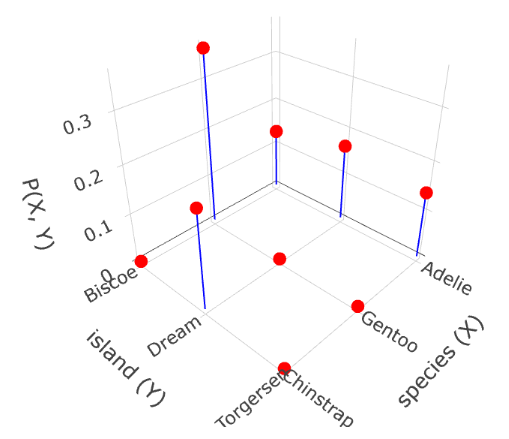
\includegraphics[width=0.7\linewidth]{SK_verzia_praca/figures/pravdeb_funk_ostrov_druhy_3D.png}
    \caption{3D znázornenie združenej pravdepodobnostnej funkcie (PMF) medzi premennými \textit{Ostrov ako miesto výskytu} a \textit{Druh} tučniakov.}
    \label{fig:miesto_druh_joint_density}
\end{figure}

Zatiaľ čo v jednorozmernom spojitom prípade nás zaujímala pravdepodobnosť výskytu náhodnej premennej v určitej oblasti na reálnej osi, v prípade dvoch spojitých premenných nás už zaujíma pravdepodobnosť, že realizácie oboch premenných spadnú do danej oblasti v rovine $\mathbb{R}^2$.

Ak $R_1 = [x_1, x_1 + dx_1]$ a $R_2 = [x_2, x_2 + dx_2]$ sú malé intervaly okolo bodu $(x_1, x_2)$, potom pravdepodobnosť, že náhodný vektor $(X_1, X_2)$ spadne do oblasti $R_1 \times R_2$, je približne:

\begin{equation}
\mathrm{Pr}(x_1 \leq X_1 \leq x_1 + dx_1,\ x_2 \leq X_2 \leq x_2 + dx_2) \approx f(x_1, x_2) \, dx_1 \, dx_2
\end{equation}

kde $f(x_1, x_2)$ je hodnota združenej hustoty pravdepodobnosti v bode $(x_1, x_2)$.

Presnejšie, pravdepodobnosť, že sa realizácie oboch premenných nachádzajú v oblasti $[a_1, b_1] \times [a_2, b_2]$, vypočítame pomocou dvojnásobného integrálu:

\begin{equation}
\mathrm{Pr}(a_1 \leq X_1 \leq b_1,\ a_2 \leq X_2 \leq b_2) = \int_{a_2}^{b_2} \int_{a_1}^{b_1} f(x_1, x_2) \, dx_1 \, dx_2
\end{equation}

Aby funkcia $f(x_1, x_2)$ bola platnou hustotou pravdepodobnosti, musí platiť:

\begin{equation}
\iint_{\mathbb{R}^2} f(x_1, x_2) \, dx_1 \, dx_2 = 1
\end{equation}

Združená hustota veľmi efektívne popisuje spoločné správanie sa dvoch spojitých náhodných premenných a tvorí základ pre ďalšie koncepty ako sú marginálne a podmienené rozdelenia.

Na nasledujúcom obrázku môžeme vidieť príklad vizualizácie združenej hustoty pravdepodobnosti homogénnej spojitej štruktúry dvoch premenných, pričom ako model výpočtu tu používame jadrové vyhladzovanie, viď ~\ref{textbf:kernel_smoothing}.

\begin{figure}[htpb]
    \centering
    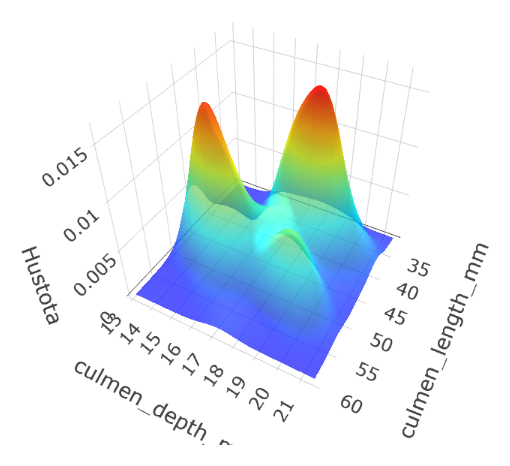
\includegraphics[width=0.7\linewidth]{hustota_hlbka_dlzka_zobaku_3D}
    \caption{3D znázornenie združenej hustoty pravdepodobnosti (PDF) medzi premennými \textit{Hĺbka zobáku} a \textit{Dĺžka zobáku} tučniakov.}
    \label{fig:zobak_joint_density}
\end{figure}

\subsection{Bodové charakteristiky}\label{joint_moments}

Rovnako ako v jednorozmernom prípade, aj v prípade viacrozmerných náhodných veličín (náhodného vektora) sú základnými charakteristikami rozdelenia \textit{stredná hodnota} a \textit{rozptyl}, pričom tentokrát si zavedieme aj pojem \textit{kovariancie}.

\subsubsection{Stredná hodnota}\label{subsubsec:joint_mean}

Pre náš dvojrozmerný náhodný vektor \(\vec{X} = (X_1, X_2)\) definujeme vektor stredných hodnôt ako:

\begin{equation}
\mathbb{E}[\vec{X}] = \left( \mathbb{E}[X_1], \mathbb{E}[X_2] \right)
\end{equation}

Pre obidva komponenty ho môžeme vyjadriť pomocou marginálnej hustoty (bližšie popísané v kapitole o marginálnom rozdelení~\ref{subsec:marginal_dist}). Napríklad pre \(X_1\) a marginálnu hustotu \(f_1(x_1)\) platí:

\begin{equation}
\mathbb{E}[X_1] = \int_{\mathbb{R}} x_1 \, f_1(x_1) \, dx_1
\end{equation}

alebo pomocou združenej hustoty:

\begin{equation}
\mathbb{E}[X_1] = \iint_{\mathbb{R}^2} x_1 \, f(x_1, x_2) \, dx_1 \, dx_2
\end{equation}

\subsubsection{Rozptyl}\label{subsubsec:joint_variance}

Rozptyl (disperzia) je definovaný ako očakávaná kvadratická odchýlka od strednej hodnoty:

\begin{equation}
\mathrm{Var}[X_1] = \mathbb{E}[(X_1 - \mathbb{E}[X_1])^2]
\end{equation}

Alternatívne možno rozptyl zapísať aj ako rozdiel momentov:

\begin{equation}
\mathrm{Var}[X_1] = \mathbb{E}[X_1^2] - (\mathbb{E}[X_1])^2
\end{equation}

\subsubsection{Kovariancia}\label{subsubsec:joint_covariance}

Kovariancia vyjadruje mieru lineárnej závislosti medzi dvoma náhodnými premennými \(X_1\) a \(X_2\). Definujeme ju ako:

\begin{equation}
\mathrm{Cov}[X_1, X_2] = \mathbb{E}[(X_1 - \mathbb{E}[X_1])(X_2 - \mathbb{E}[X_2])]
\end{equation}

Kovariancia sa dá alternatívne vyjadriť aj pomocou spoločného momentu:

\begin{equation}
\mathrm{Cov}[X_1, X_2] = \mathbb{E}[X_1 X_2] - \mathbb{E}[X_1] \cdot \mathbb{E}[X_2]
\end{equation}

Tieto hodnoty sa sumarizujú do dvojdimenzionálnej \textit{kovariančnej matice} \(\Sigma\), ktorá je symetrická a pozitívne semidefinitná:

\begin{equation}
\Sigma = 
\begin{bmatrix}
\mathrm{Var}[X_1] & \mathrm{Cov}[X_1, X_2] \\
\mathrm{Cov}[X_2, X_1] & \mathrm{Var}[X_2] \\
\end{bmatrix}
\end{equation}

Kovariančná matica je nevyhnutným nástrojom pre analýzu rozptylu a závislostí medzi komponentami náhodného vektora. Využíva sa napríklad pri odhade parametrov v lineárnej regresii alebo v diskriminačnej analýze.

\subsection{Marginálne rozdelenie}\label{subsec:marginal_dist}

Ak nás nezaujíma spoločné správanie všetkých náhodných premenných vektorovej premennej $\vec{X} = (X_1, X_2)$, ale iba jedného jej komponentu, môžeme skúmať jej vlastné pravdepodobnostné rozdelenie. Takéto rozdelenie nazývame \textit{marginálne rozdelenie} (angl. marginal distribution).

Na vizualizáciu marginálneho rozdelenia danej premennej, napríklad $X_2$, môžeme premietnuť každý bod z roviny $(x_1, x_2)$ na os $x_2$ a zostrojiť tak histogram týchto projekcií. Výsledný histogram, po normalizácii tak, aby plocha všetkých stĺpcov bola rovná 1, poskytuje empirický odhad marginálnej hustoty $f_2(x_2)$.

\begin{figure}[H] 
    \centering 
    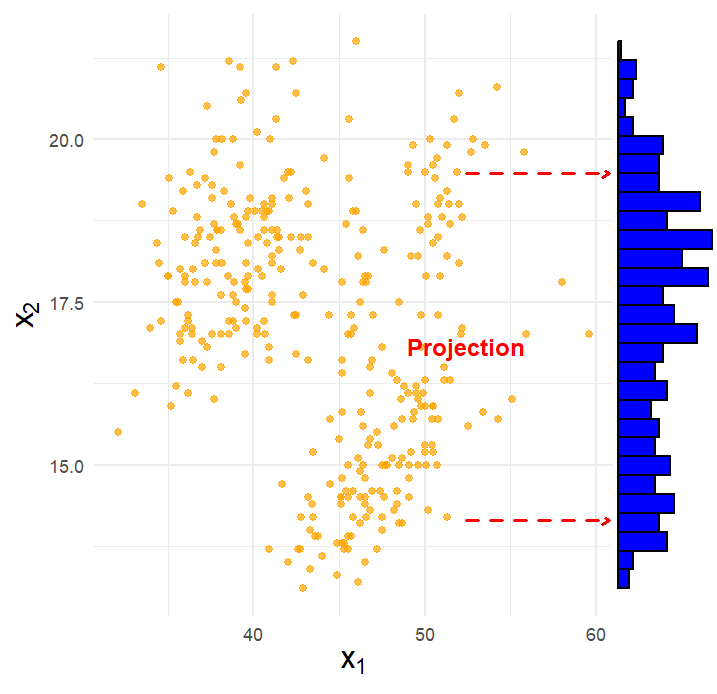
\includegraphics[width=0.7\linewidth]{marg_proj_hist.png} 
    \caption{Empirický odhad marginálneho rozdelenia $f_2(x_2)$} 
    \label{fig:margin_proj} 
\end{figure}

Z iného pohľadu, marginálne rozdelenie premennej $X_2$ vyjadruje pravdepodobnosť, že hodnota $X_2$ spadne do veľmi úzkeho intervalu $[x_2, x_2 + dx_2]$. V kontexte dvojrozmerného bodového grafu to zodpovedá pravdepodobnosti, že sa bod $(x_1, x_2)$ nachádza v horizontálnom páse výšky $dx_2$.

\begin{figure}[H]
    \centering
    \begin{subfigure}[b]{0.48\linewidth}
        \centering
        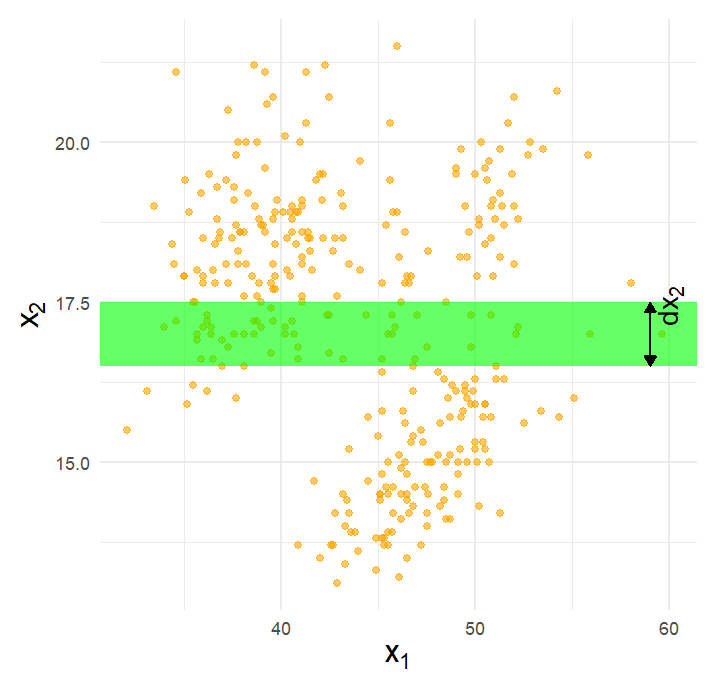
\includegraphics[width=\linewidth]{marg_strip_sum1.png}
        \caption{Horizontálny pás šírky $dx_2$ reprezentujúci interval pre $X_2$.}
        \label{fig:marg_strip_a}
    \end{subfigure}
    \hfill
    \begin{subfigure}[b]{0.48\linewidth}
        \centering
        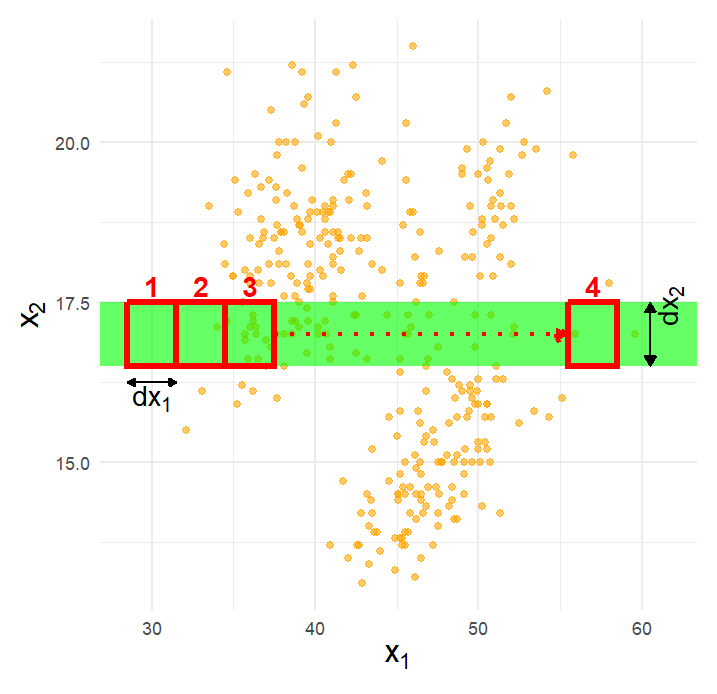
\includegraphics[width=\linewidth]{marg_strip_sum2.png}
        \caption{Pás rozdelený na plôšky $dx_1 \cdot dx_2$, z ktorých sa skladá marginálne rozdelenie $f_2(x_2)$.}
        \label{fig:marg_strip_b}
    \end{subfigure}
    \caption{Vizuálna interpretácia marginálneho rozdelenia $f_2(x_2)$}
    \label{fig:marg_strip}
\end{figure}

Ak si pás rozdelíme na plôšky $dx_1 \cdot dx_2$  (Obr.~\ref{fig:marg_strip_b}), potom z nich váženým súčtom dostaneme:

\begin{equation}
\mathrm{Pr}(x_2 \leq X_2 \leq x_2 + dx_2) \approx \sum_i f(x_1^{(i)}, x_2) \, dx_1 \, dx_2
\end{equation}

Porovnaním so vzťahom pre jednorozmernú hustotu pre spojité premenné nám vychádza vzťah, ktorý hovorí o tom, že marginálne rozdelenie $X_2$ možno získať z hustoty združeného rozdelenia $f(x_1, x_2)$ integráciou cez všetky hodnoty $x_1$:

\begin{equation} f_2(x_2) = \int_{-\infty}^{\infty} f(x_1, x_2) dx_1 \end{equation}

Podobne marginálne rozdelenie premennej $X_1$ získame ako:

\begin{equation} f_1(x_1) = \int_{-\infty}^{\infty} f(x_1, x_2)  dx_2 \end{equation}

Tieto marginálne rozdelenia slúžia ako základ pre rozklad združeného rozdelenia pomocou kopúl, ktorý bude predmetom nasledujúcej podkapitoly.

\begin{figure}[H]
    \centering
    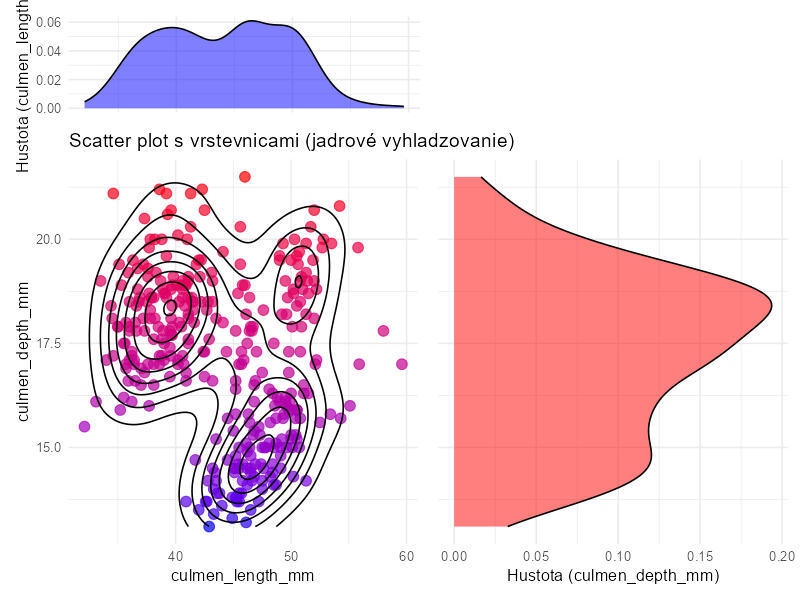
\includegraphics[width=0.8\linewidth]{hustota_hlbka_dlzka_zobaku_2D}
    \caption{Vrstevnice združenej PDF(Obr.~\ref{fig:zobak_joint_density}) + po bokoch marginálne PDF premenných \textit{Hĺbka zobáku} a \textit{Dĺžka zobáku} tučniakov (metóda: jadrové vyhladzovanie ~\ref{textbf:kernel_smoothing})}
    \label{fig:zobak_marg_density}
\end{figure}

\subsection{Podmienené rozdelenie}\label{subsec:conditional_distribution}

Kým marginálne rozdelenie opisuje správanie jednej premennej bez toho aby sa bral do úvahy vplyv ostatných premenných na túto premennú, v mnohých praktických situáciách nás zaujíma, ako sa rozdelenie jednej premennej mení v závislosti od známych hodnôt inej premennej. V takýchto prípadoch hovoríme o \textit{podmienenom rozdelení}.

\subsubsection{Hustota}\label{subsubsec:conditional_density}

Formálne, ak máme náhodný vektor $(X_1, X_2)$, potom podmienená hustota premennej $X_2$ vzhľadom na známu hodnotu $X_1 = x_1$ je definovaná ako:

\begin{equation}
f_{2 \mid 1}(x_2 \mid x_1) = \frac{f(x_1, x_2)}{f_1(x_1)},
\end{equation}

kde:
\begin{itemize}
  \item $f(x_1, x_2)$ je združená hustota,
  \item $f_1(x_1) = \int_{-\infty}^{\infty} f(x_1, x_2) \, dx_2$ je marginálna hustota premennej $X_1$.
\end{itemize}

Z definície o podmienenej pravdepodobnosti vyplýva:

\begin{equation}
\mathrm{Pr}(a \leq X_2 \leq b \mid X_1 = x_1) = \int_a^b f_{2 \mid 1}(x_2 \mid x_1) \, dx_2.
\end{equation}

Podmienenú hustotu tu taktiež možno intuitívne interpretovať ako hustotu v rámci tenkého vertikálneho pásu, kde náhodná premenná $X_1$ nadobúda hodnoty z intervalu $[x, x + \varepsilon]$ (Obr.~\ref{fig:cond_density_strip}). V tomto pásme vyberieme všetky body, ktoré spadajú do intervalu $[x, x + \varepsilon]$, a z nich vytvoríme histogram hodnôt premennej $X_2$, čím získame empirický odhad hustoty $f_{2 \mid 1}(x_2 \mid X_1 = x)$.

Tento postup je znázornený na nasledujúcom obrázku:

\begin{figure}[H]
    \centering
    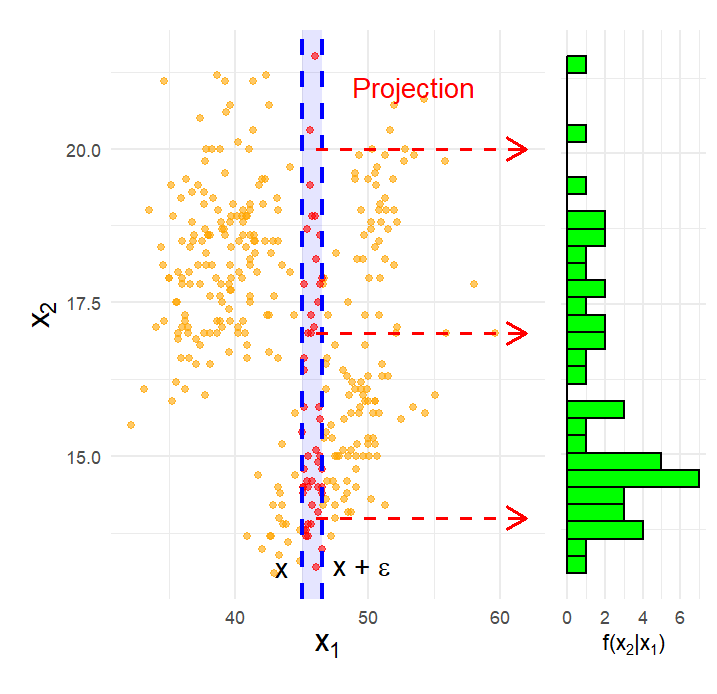
\includegraphics[width=0.7\linewidth]{marg_condition_strip.png}
    \caption{Empirický odhad podmienenej hustoty $f_{2 \mid 1}(x_2 \mid x_1 \in [x, x + \epsilon])$}
    \label{fig:cond_density_strip}
\end{figure}

Týmto sme zaviedli pojem podmienenej hustoty, ktorý bude ďalej kľúčový pri výpočte tzv. \textit{podmienenej strednej hodnoty}.

\subsubsection{Podmienená stredná hodnota}\label{subsubsec:conditional_mean}

\section{Rozklad}\label{sec:rozklad_kopule}
\section{Odhad}\label{sec:odhad}
        \chapter{Modelovanie rozdelenia zmiešaného náhodného vektora}\label{sec:joint_mixture_dist}


        \chapter{Aplikácie}\label{sec:applications}


	\chapter{Záver}

V závere zhrniete, čomu sa venovala vaša práca, ako sa vám podarilo naplniť stanovené ciele a k akým výsledkom ste prišli. Môžete zhodnotiť váš postup riešenia problému, jeho výhody/nevýhody. V závere je vhodné aj naznačiť, akými smermi by sa dalo v práci pokračovať, aké zostali nevyriešené otázky, kde vidíte možnosti vylepšenia a podobne.


	% ====== Bibliografia a prilohy ======
%	\nocite{*} % Vypise v bibliografii aj zroje, ktore neboli citovane
	\printbibliography[heading=bibintoc]
	
	\chapter*{Použitie umelej inteligencie}
\addcontentsline{toc}{chapter}{Použitie umelej inteligencie}

Od 1.12.2024 je v platnosti predpis \uv{Používanie umelej inteligencie na STU
v Bratislave}, nájdete ho aj v priečinku \verb|ZaverecnaPracaMPM\dokumenty|. Predpis sa týka aj záverečných prác. Ak ste použili AI, treba to v práci na tomto mieste deklarovať a uviesť podrobnosti. Niekoľko príkladov (uvedených v predpise) je tu:

\begin{itemize}
	\item \textit{OpenAI (2024), ChatGPT, časť 2.1, generovanie textu}
	
	\item \textit{OpenAI (2024), ChatGPT, časť 5.4, generovanie kódu na vizualizáciu výsledkov, jazyk Pyton}
	
	\item \textit{Google, Geminy (2024), získanie experimentálnych dát pre experiment v časti 7.2.3}
	
	\item \textit{DeepL (2024), https://www.deepl.com/en/translator, preklady viacerých častí textu}
	
	\item \textit{Grammarly, https://app.grammarly.com, gramatická korekcia celého textu}
\end{itemize}
	
	
	%\includepdf[pages=-,pagecommand={}]{documents/priloha1.pdf} % pripadne prilohy
\end{document}